%% ============================================================
%%  STANDARD PREAMBLE (article, lecture notes)
%% ============================================================

% ---------- Document class and page layout ----------
\documentclass[11pt]{article}      % Basic document type, 11pt body text
\usepackage[margin=1in]{geometry}  % Sets page margins to 1 inch on all sides

% ---------- Math ----------
\usepackage{amsmath,amssymb}       % Core math: align, cases, \text{}, plus extra symbols (\mathbb, \hbar, ...)

% ---------- Colors and boxes ----------
\usepackage{xcolor}                % Lets you use colors (\textcolor{red}{...})
\usepackage{mdframed}              % Boxes around text that can break across pages (theorems, key results)

% ---------- Diagrams ----------
\usepackage{tikz-cd}               % Commutative diagrams / arrow diagrams (also loads tikz)
\usepackage{tikz}                  % General-purpose drawing: lines, shapes, plots
\usetikzlibrary{arrows.meta, positioning} % arrows.meta: more arrow tip styles; positioning: place nodes "right=of A"

% ---------- Text layout ----------
\usepackage{multicol}              % Multi-column text (\begin{multicols}{2} ... \end{multicols})
\usepackage{indentfirst}           % Indents the first paragraph after a heading (article class skips it by default)

% ---------- Hyperlinks ----------
\usepackage[hidelinks]{hyperref}   % Clickable TOC, \ref, \eqref, \cite; hidelinks = no colored text or boxes

% ---------- Equation numbering ----------
\numberwithin{equation}{section}   % Equation counter resets in each section
\renewcommand{\theequation}{\thesection.\arabic{equation}} % Displays numbers as section.equation, e.g. (2.3)

% ---------- Paragraph style ----------
\setlength{\parindent}{2em}        % First-line indent of each paragraph
\setlength{\parskip}{1\baselineskip} % Extra vertical gap between paragraphs

% ---------- Title block ----------
\title{Statistical Mechanics rediscovered under the lense of entropy maximization principles}
\author{Duy M. Dao}
\date{\today}                      % Compile date; replace with a fixed date if you prefer

\begin{document}
\maketitle                         % Prints title, author, date
\tableofcontents                   % Clickable table of contents

\newpage
\part{Statistical Derivation of Ensembles}
    \section{Entropy Maximization Principle}

\paragraph{The conventional approach and its limitation.}
The conventional introduction to statistical mechanics rests on four notions:
\begin{itemize}
    \item A \textcolor{blue}{microstate} is a complete description of every
    microscopic parameter of the system.
    \item In an isolated system, all microstates are equally likely.
    \item A \textcolor{blue}{macrostate} is a group of microstates that share
    the same macroscopic observables.
    \item Macrostates that contain more microstates are observed more often,
    so the observed macrostate is the most probable one.
\end{itemize}
Boltzmann, Gibbs, and other founders of thermodynamics developed this
approach. It is physically intuitive, but explaining why a system settles
into the most probable macrostate requires \textcolor{blue}{ergodicity} and
dynamical arguments, which are difficult to make rigorous.

\paragraph{The MaxEnt alternative.}
In this document, we follow Jaynes and treat equilibrium statistical
mechanics as the solution of a constrained optimization problem: maximize
the entropy subject to what is macroscopically known about the system. We
call this the \textcolor{blue}{Entropy Maximization Principle (MaxEnt)}.

\subsection{Gibbs-Shannon Entropy}

\paragraph{From ``disorder'' to ignorance.}
The meaning of \textcolor{blue}{entropy} has long been debated. The popular
description of entropy as ``disorder'' is not a definition, because it gives
no quantitative way to measure disorder. Clausius, Boltzmann, and other
founders regarded entropy as a driving force of thermodynamic processes, which
left open the question of which physical quantity entropy encodes. Jaynes
proposed instead that entropy is not a property of the body itself, but a
measure of our \textcolor{blue}{ignorance} about it. The
\textcolor{blue}{Gibbs-Shannon entropy} formalizes this idea for $\Omega$
events that occur with probabilities $p(i)$:
\begin{equation}
    \boxed{S(p) = -\sum_{i=1}^{\Omega} p(i)\ln p(i).}
\end{equation}

\paragraph{Why the Gibbs-Shannon entropy measures ignorance.}
The term $-\ln p(i)$ measures our ignorance about event $i$, also called its
\textcolor{blue}{surprisal}:
\begin{itemize}
    \item A certain event has $p(i)=1$, so its ignorance is $-\ln 1 = 0$.
    \item A rare event has small $p(i)$, so its ignorance is large.
\end{itemize}
Summing $-\ln p(i)$ directly would fail, because knowing that an event will
occur and knowing that it will not occur both mean low ignorance. We
therefore weight each term by $p(i)$. Rare events seldom occur, and
near-certain events are already expected, so both contribute little to the
total. Equivalently, $S$ is the expected value of $-\ln p$.

\subsection{Entropy Maximization}

\paragraph{The principle of maximum ignorance.}
Jaynes' second idea is that, without knowledge of the underlying mechanism,
we should choose the distribution that maximizes our ignorance, that is, the
Gibbs-Shannon entropy $S(p)$, subject to the known constraints. A
lower-entropy distribution would introduce an unexplained bias toward some
events. For example, a coin flip should assign equal probabilities to both
outcomes unless a constraint, such as a loaded coin, states otherwise.

\paragraph{Formulating the constrained optimization.}
\textcolor{red}{For simplicity, we write $p_i$ instead of $p(i)$ from now on,
as there is no need to distinguish between different probability
distributions.}
We write each known constraint as $g_a(p)=0$. For the expectation value of an
observable with value $g_a(i)$ in event $i$,
\begin{equation*}
    g_a(p) = \sum_i p_i\, g_a(i) - \langle g_a\rangle .
\end{equation*}
Lagrange multipliers remove the constraints. We define the Lagrangian
\begin{equation}
    \boxed{\mathcal{L}(p)
    = -\sum_i p_i \ln p_i
    - \alpha\left(\sum_i p_i - 1\right)
    - \sum_a \lambda_a\, g_a(p),}
\end{equation}
where $\alpha$ enforces normalization and each $\lambda_a$ enforces one
constraint. The maximizing distribution satisfies
\begin{equation}
    \boxed{\frac{\partial \mathcal{L}}{\partial p_i} = 0,
    \qquad
    \frac{\partial \mathcal{L}}{\partial \alpha} = 0,
    \qquad
    \frac{\partial \mathcal{L}}{\partial \lambda_a} = 0.}
    \label{eq:conditions}
\end{equation}
The last two conditions reproduce normalization and the constraints. The
first condition determines $p_i$.

% ---------- Optional: general solution, makes later ensembles special cases ----------
\paragraph{The general MaxEnt distribution.}
For expectation-value constraints, $\partial g_a/\partial p_i = g_a(i)$. The
first condition in Eq.~\eqref{eq:conditions} then gives
\begin{align*}
    -\ln p_i - 1 - \alpha - \sum_a \lambda_a\, g_a(i) &= 0, \\
    p_i &= e^{-1-\alpha}\, \exp\!\Big(-\sum_a \lambda_a\, g_a(i)\Big).
\end{align*}
Normalization fixes $\alpha$ and yields
\begin{equation}
    \boxed{p_i = \frac{1}{Z}\exp\!\Big(-\sum_a \lambda_a\, g_a(i)\Big),
    \qquad
    Z = \sum_i \exp\!\Big(-\sum_a \lambda_a\, g_a(i)\Big).}
\end{equation}
Since $S$ is strictly concave in $p$ and the constraints are linear, this
stationary point is the unique maximum.                % Each \include starts on a new page
    \section{The Microcanonical Ensemble}

\paragraph{The Boltzmann constant in the entropy.}
In thermodynamics, the Gibbs-Shannon entropy carries the Boltzmann constant
$k_B$, which sets the units of entropy:
\begin{equation}
    \boxed{S(p) = -k_B\sum_{i=1}^{\Omega} p_i\ln p_i.}
\end{equation}
\textcolor{red}{For simplicity, we set $k_B=1$ during derivations and restore
it when stating final results.}

\paragraph{From normalization alone to Boltzmann's entropy.}
We first consider the simplest case, in which the only constraint is
normalization, $\sum_i p_i=1$. This case describes the
\textcolor{blue}{microcanonical ensemble}: an isolated system with fixed
energy and other fixed macroscopic constraints. The energy is not imposed
through a Lagrange multiplier. Instead, it restricts the sample space to the
microstates with energy $U$, in practice a thin shell $[U,U+\delta U]$.
Setting the derivatives of the Lagrangian in Eq.~\eqref{eq:conditions} to
zero gives
\begin{align*}
    \frac{\partial\mathcal{L}}{\partial p_i} = -\ln p_i-1-\alpha = 0,
    \qquad
    \frac{\partial\mathcal{L}}{\partial\alpha} = -\Big(\sum_i p_i-1\Big) = 0.
\end{align*}
The first condition gives $p_i=e^{-1-\alpha}$, which does not depend on $i$.
Normalization then requires $\Omega\, e^{-1-\alpha}=1$, so
\begin{equation}
    \boxed{p_i = \frac{1}{\Omega}.}
\end{equation}
Maximizing the entropy under normalization alone therefore yields a uniform
distribution: all accessible microstates are equally probable. The
conventional approach postulates this property. Here, MaxEnt derives it, and
it recovers Boltzmann's premise for the microcanonical ensemble. Substituting
$p_i=1/\Omega$ into the entropy gives
\begin{align*}
    S = -\sum_{i=1}^{\Omega}\frac{1}{\Omega}\ln\frac{1}{\Omega} = \ln\Omega,
\end{align*}
and restoring $k_B$ yields Boltzmann's microcanonical entropy:
\begin{equation}
    \boxed{S = k_B\ln\Omega.}
\end{equation}

\paragraph{Dependence of the entropy on the macroscopic constraints.}
The number of accessible microstates, $\Omega$, is also called the
\textcolor{blue}{microcanonical partition function}. It depends on the
system's Hamiltonian $\mathcal{H}$ and on the macroscopic constraints. In
particular, the accessible microstates are set by the volume $V$, the
particle number $N$, and the internal energy $U$, so the entropy is a
function of these three variables:
\begin{equation}
    \boxed{S = S(N,V,U).}
\end{equation}
Specifying $N$, $V$, and $U$ therefore determines the equilibrium entropy
uniquely.
    \section{The Canonical Ensemble}

\paragraph{Constraining the average of an observable.}
The microcanonical ensemble does not distinguish between accessible
microstates: only their number matters. Realistic systems, however, obey
constraints imposed by measurement. Suppose microstate $i$ has a definite
value $a_i$ of an observable $A$, and the measured average is $\bar A$. The
expectation value is
\begin{equation}
    \boxed{\langle A\rangle \equiv \sum_i p_i a_i,}
\end{equation}
and the constraint reads $\langle A\rangle=\bar A$.
\textcolor{red}{Here, $\langle A\rangle$ denotes the operation that extracts
the mean of the observable $A$, and $\bar A$ denotes the numerical value
assigned to that mean. Since only one constraint is present, we also rename
the multiplier $\lambda_a$ as $\beta$.}
The Lagrangian now contains the multiplier $\alpha$ for normalization and
the multiplier $\beta$ for the constraint on $\langle A\rangle$. Its
stationarity conditions are
\begin{align*}
    \frac{\partial\mathcal{L}}{\partial p_i}
    &= -\ln p_i-1-\alpha-\beta a_i=0, \\
    \frac{\partial\mathcal{L}}{\partial\alpha}
    &= -\Big(\sum_i p_i-1\Big)=0, \\
    \frac{\partial\mathcal{L}}{\partial\beta}
    &= -\Big(\sum_i a_i p_i-\bar A\Big)=0.
\end{align*}

\paragraph{The Boltzmann distribution and the partition function.}
The first condition gives $p_i = e^{-1-\alpha-\beta a_i}$. Substituting this
into normalization and into the constraint yields
\begin{align*}
    e^{-1-\alpha}\sum_i e^{-\beta a_i} = 1,
    \qquad
    e^{-1-\alpha}\sum_i a_i e^{-\beta a_i} = \bar A.
\end{align*}
The first equation determines $\alpha$ in terms of $\beta$ and leaves a
single free parameter. Defining the \textcolor{blue}{canonical partition
function}
\begin{equation}
    \boxed{Z(\beta) \equiv \sum_i e^{-\beta a_i},}
\end{equation}
the probability distribution becomes
\begin{equation}
    \boxed{p_i = \frac{e^{-\beta a_i}}{Z(\beta)}.}
\end{equation}
This is the \textcolor{blue}{Boltzmann distribution}. For $\beta>0$, states
with larger $a_i$ are less probable. The remaining constraint,
$\langle A\rangle(\beta)=\bar A$, determines $\beta$.

\paragraph{Uniqueness of the multiplier.}
To show that $\beta$ is unique, we first express the mean through $Z$:
\begin{align*}
    \langle A\rangle = \frac{1}{Z}\sum_i a_i e^{-\beta a_i}
    = -\frac{\partial\ln Z}{\partial\beta}.
\end{align*}
Hence
\begin{equation}
    \boxed{\langle A\rangle = -\frac{\partial\ln Z}{\partial\beta}.}
\end{equation}
Differentiating once more, with $\mathrm{Var}(A)\equiv\langle A^2\rangle-\langle A\rangle^2$,
\begin{align*}
    \frac{\partial\langle A\rangle}{\partial\beta}
    &= \frac{\partial}{\partial\beta}
    \left(\frac{\sum_i a_i e^{-\beta a_i}}{Z}\right) \\
    &= -\frac{\sum_i a_i^2 e^{-\beta a_i}}{Z}
    +\frac{1}{Z^2}\left(\sum_i a_i e^{-\beta a_i}\right)^2 \\
    &= -\langle A^2\rangle+\langle A\rangle^2
    = -\mathrm{Var}(A),
\end{align*}
so
\begin{equation}
    \boxed{\frac{\partial\langle A\rangle}{\partial\beta} = -\mathrm{Var}(A).}
\end{equation}
Since $\mathrm{Var}(A)\geq0$, $\langle A\rangle(\beta)$ is monotonically
non-increasing. It is strictly decreasing whenever $A$ is not identical
across all accessible microstates. Thus, for target values in the interior
of the achievable range, $\langle A\rangle$ determines $\beta$ uniquely.

\paragraph{Entropy of the canonical distribution and the meaning of $\beta$.}
We now compute the entropy of the resulting distribution, with $k_B$
omitted during the derivation:
\begin{align*}
    S &= -\sum_i p_i\ln p_i
    = -\sum_i p_i\left(-\beta a_i-\ln Z\right) \\
    &= \beta\sum_i a_i p_i+\ln Z\sum_i p_i
    = \beta\langle A\rangle+\ln Z.
\end{align*}
Restoring $k_B$,
\begin{equation}
    \boxed{S=k_B\left(\beta\langle A\rangle+\ln Z\right).}
\end{equation}
Although $S$ depends on $\bar A$ both explicitly and implicitly through
$\beta(\bar A)$, differentiating gives
\begin{align*}
    \frac{\partial S}{\partial\langle A\rangle}
    &= \beta
    +\langle A\rangle\frac{d\beta}{d\langle A\rangle}
    +\frac{\partial\ln Z}{\partial\beta}\frac{d\beta}{d\langle A\rangle} \\
    &= \beta
    +\langle A\rangle\frac{d\beta}{d\langle A\rangle}
    -\langle A\rangle\frac{d\beta}{d\langle A\rangle}
    = \beta.
\end{align*}
Restoring $k_B$ yields the meaning of the multiplier:
\begin{equation}
    \boxed{\beta=\frac{1}{k_B}\frac{\partial S}{\partial\langle A\rangle}.}
\end{equation}

\paragraph{Concavity of the entropy.}
A function $f$ is \textcolor{blue}{concave} on an interval $I$ if, for all
$x,y\in I$ and all $t\in[0,1]$,
\begin{equation}
    \boxed{f\big(tx+(1-t)y\big)\;\geq\;t\,f(x)+(1-t)\,f(y).}
\end{equation}
Geometrically, every chord lies on or below the graph. The function is
\textcolor{blue}{strictly concave} if the inequality is strict for $x\neq y$
and $t\in(0,1)$. For a twice-differentiable $f$, concavity is equivalent to
$f''\leq0$, and $f''<0$ guarantees strict concavity.

We apply this criterion to $S$ as a function of $\langle A\rangle$. Using
the inverse-function rule and $\partial\langle A\rangle/\partial\beta=-\mathrm{Var}(A)$,
\begin{align*}
    \frac{\partial^2 S}{\partial\langle A\rangle^2}
    = \frac{d\beta}{d\langle A\rangle}
    = \left(\frac{d\langle A\rangle}{d\beta}\right)^{-1}
    = -\frac{1}{\mathrm{Var}(A)}.
\end{align*}
Restoring $k_B$,
\begin{equation}
    \boxed{\frac{\partial^2 S}{\partial\langle A\rangle^2}
    = -\frac{k_B}{\mathrm{Var}(A)}<0.}
\end{equation}
The entropy is therefore strictly concave in $\langle A\rangle$ whenever $A$
is not identical across all accessible microstates. This is the monotonic
decrease of $\langle A\rangle(\beta)$ read from the side of $S$: each value
of $\langle A\rangle$ corresponds to exactly one $\beta$.

\paragraph{Specialization to the internal energy.}
We have not specified the observable $A$, so the derivation applies to any
observable whose expectation value is constrained. The canonical ensemble
conventionally fixes the volume $V$ and particle number $N$ and constrains
the internal energy. \textcolor{red}{From here on, we take $A=U$ and write
$U_i$ for $a_i$.} The results become
\begin{equation}
    \boxed{
    \begin{aligned}
        Z(\beta) &= \sum_i e^{-\beta U_i}, &
        p_i &= \frac{e^{-\beta U_i}}{Z(\beta)}, \\
        \langle U\rangle &= -\frac{\partial\ln Z}{\partial\beta}, &
        S &= k_B\left(\beta\langle U\rangle+\ln Z\right).
    \end{aligned}}
\end{equation}
We identify $\beta$ with the temperature in Section~\ref{sec:multipliers}.
The reason for not constraining only the particle number or the volume will
be discussed shortly.

\paragraph{Recovering the microcanonical ensemble.}
If every accessible microstate has the same energy $U$, the canonical
ensemble reduces to the microcanonical one. All weights $e^{-\beta U}$ are
identical, so the distribution is uniform and the mean energy is the exact
value $U$. Then
\begin{align*}
    Z &= \sum_{i=1}^{\Omega} e^{-\beta U} = \Omega\, e^{-\beta U}, \\
    S &= k_B\left(\beta U+\ln\Omega-\beta U\right) = k_B\ln\Omega.
\end{align*}

\subsection{First and Second Law of Thermodynamics - Making Sense of Multipliers}
\label{sec:multipliers}

\paragraph{The multipliers need thermodynamics for their meaning.}
The MaxEnt formalism does not by itself provide the physical interpretation
or numerical calibration of its multipliers. In particular, the
identification
\begin{equation}
    \boxed{\beta=\frac{1}{k_B}\frac{\partial S}{\partial \langle U\rangle}=\frac{1}{k_BT}}
\end{equation}
cannot be derived from MaxEnt alone. It is an empirical correspondence
established by classical thermodynamics. We therefore obtain the physical
meaning of the multipliers by connecting them to the thermodynamic laws.

\paragraph{From the first and second laws to the fundamental relation.}
The \textcolor{blue}{first law} expresses energy conservation:
\begin{equation}
    \boxed{dU = \delta Q-\delta W+\mu\, dN,}
\end{equation}
where
\begin{itemize}
    \item $\delta W=P\,dV$ is the work done \emph{by} the system.
    \item The symbols $\delta Q$ and $\delta W$ emphasize that heat and work
    are not state functions: their values depend on the path between two
    states.
    \item The \textcolor{blue}{chemical potential} $\mu$ is the change in
    internal energy associated with adding particles at fixed entropy and
    volume.
\end{itemize}
The \textcolor{blue}{second law}, in the form of the Clausius inequality,
states
\begin{equation}
    \boxed{\delta Q\leq T\,dS,}
\end{equation}
with equality for reversible processes. Combining the two laws for a
reversible process gives
\begin{equation}
    \boxed{dU=T\,dS-P\,dV+\mu\, dN,}
    \label{eq:combined-law}
\end{equation}
and therefore
\begin{equation}
    \boxed{
    \frac{\partial U}{\partial S}\bigg|_{V,N}=T, \qquad
    \frac{\partial U}{\partial V}\bigg|_{S,N}=-P, \qquad
    \frac{\partial U}{\partial N}\bigg|_{S,V}=\mu.}
    \label{eq:U-derivs}
\end{equation}
Rearranging Eq.~\eqref{eq:combined-law} gives the equivalent form
\begin{equation}
    \boxed{dS=\frac{1}{T}\,dU+\frac{P}{T}\,dV-\frac{\mu}{T}\,dN,}
\end{equation}
and therefore
\begin{equation}
    \boxed{
    \frac{\partial S}{\partial U}\bigg|_{V,N}=\frac{1}{T}, \qquad
    \frac{\partial S}{\partial V}\bigg|_{U,N}=\frac{P}{T}, \qquad
    \frac{\partial S}{\partial N}\bigg|_{U,V}=-\frac{\mu}{T}.}
    \label{eq:S-derivs}
\end{equation}

\subsection{Extensive and Intensive Variables}

\paragraph{Extensive and intensive variables and their conjugate pairs.}
\begin{itemize}
    \item A quantity $X$ is \textcolor{blue}{extensive} if, for two weakly
    coupled subsystems, $X_{\mathrm{total}}=X_1+X_2$. Equivalently, for
    $\lambda$ identical, non-interacting copies, $X_\lambda=\lambda X_1$.
    \item A quantity $Y$ is \textcolor{blue}{intensive} if it does not scale
    with the number of copies: $Y_\lambda=Y_1$.
    \item Energy, particle number, volume, and entropy are extensive, while
    temperature, pressure, and chemical potential are intensive.
\end{itemize}
This distinction explains why the Lagrange multipliers associated with
extensive constraints are intensive. For any observable $A$ with constrained
average $\langle A\rangle$, the multiplier is
\begin{equation*}
    \beta_A\equiv\frac{1}{k_B}\frac{\partial S}{\partial\langle A\rangle}.
\end{equation*}
Because $\langle A\rangle$ and $S$ are both extensive, their scaling factors
cancel in the derivative, so $\beta_A$ is intensive. Thermodynamic variables
therefore come in \textcolor{blue}{conjugate pairs}: an extensive variable
and its \textcolor{blue}{intensive conjugate}.

\paragraph{Additivity of entropy follows from statistical independence.}
\textcolor{red}{Here, the superscripts $(1)$ and $(2)$ also label the
distributions of the two systems, $p^{(1)}_i$ and $p^{(2)}_j$.}
The partition function factorizes because the joint distribution does:
$p_{ij}=p^{(1)}_i\,p^{(2)}_j$. The entropy is then additive:
\begin{align*}
    S_{1+2}
    = -\sum_{i,j} p^{(1)}_i p^{(2)}_j
    \ln\!\big(p^{(1)}_i p^{(2)}_j\big)
    = S_1+S_2.
\end{align*}
This requires statistical independence, not equilibrium, so the two systems
may have different multipliers $\beta_1$ and $\beta_2$:
\begin{equation}
    \boxed{S_{1+2}=k_B\left(\beta_1\langle U_1\rangle+\ln Z_1
    +\beta_2\langle U_2\rangle+\ln Z_2\right).}
\end{equation}
Only when $\beta_1=\beta_2=\beta$, that is, when the two systems are in
thermal equilibrium, does the joint system become canonical with a single
multiplier:
\begin{equation}
    \boxed{S_{1+2}=k_B\left[\beta\langle U_{1+2}\rangle+\ln Z_{1+2}\right],
    \qquad U_{1+2}=U_1+U_2.}
\end{equation}
Independence holds when the coupling between the systems is weak. For strong
coupling, the joint distribution does not factorize, and
$S_{1+2}=S_1+S_2-I$ with the mutual information $I\geq0$.

\subsection{Energy Fluctuation, Thermodynamic Limit, and Equivalence of Ensembles}

\paragraph{Energy fluctuation and the heat capacity.}
The variance of the internal energy, the \textcolor{blue}{energy
fluctuation} around the controlled mean $\langle U\rangle=\bar U$, can be
written in familiar thermodynamic quantities. By the chain rule,
\begin{align*}
    \mathrm{Var}(U)
    = -\frac{\partial\langle U\rangle}{\partial\beta}
    = -\frac{\partial\langle U\rangle}{\partial T}\frac{\partial T}{\partial\beta}.
\end{align*}
Since $T=1/(k_B\beta)$, we have $\partial T/\partial\beta=-k_BT^2$. By
definition, $\left.\partial\langle U\rangle/\partial T\right|_{V,N}\equiv C_V$
is the \textcolor{blue}{isochoric heat capacity}. It is computed at fixed
volume and particle number, which are the natural variables of the canonical
ensemble. Substituting,
\begin{equation}
    \boxed{\mathrm{Var}(U) = k_B T^2\, C_V.}
\end{equation}

\paragraph{Why fluctuations vanish in the thermodynamic limit.}
One might attribute the smallness of fluctuations to the tiny numerical
value of $k_B$ in SI units. This is not the reason: the value of $k_B$ only
reflects our choice of units. The genuine reason is that $C_V$ and
$\langle U\rangle$ are both extensive and scale linearly with the particle
number $N$. Hence
\begin{equation}
    \boxed{\frac{\sqrt{\mathrm{Var}(U)}}{\langle U\rangle}
    \sim\frac{\sqrt{N}}{N}=\frac{1}{\sqrt{N}},}
\end{equation}
which vanishes as $N\to\infty$. For a macroscopic system, relative energy
fluctuations are negligible because of the sheer size of $N$.
\textcolor{red}{For this reason, we write $U$ in place of $\langle U\rangle$
from here on, and likewise for other extensive variables.}
At large $N$, the canonical ensemble therefore behaves as the microcanonical
one: the fluctuation is negligible, and the relation between energy and
temperature is one-to-one.

\paragraph{Physical reading of the fluctuation formula.}
At higher temperature, $\beta$ is smaller, so the entropic cost per unit of
exchanged energy is smaller. The system then absorbs or releases energy more
freely, consistent with the larger fluctuation $k_BT^2C_V$.

\paragraph{Concavity of $S(U)$ and thermodynamic stability.}
Applying the concavity result to $A=U$ and using $\mathrm{Var}(U)=k_BT^2C_V$,
\begin{equation}
    \boxed{\frac{\partial^2 S}{\partial U^2}
    = -\frac{k_B}{\mathrm{Var}(U)} = -\frac{1}{C_V\,T^2}.}
\end{equation}
Concavity of $S(U)$ is therefore equivalent to $C_V>0$, the
\textcolor{blue}{thermodynamic stability} condition: adding energy to a
system must raise its temperature. This property is needed again when we
introduce Legendre transformations.

\subsection{Zeroth Law of Thermodynamics}

\paragraph{Two bodies exchanging energy.}
Consider two bodies, $(1)$ and $(2)$, in contact so that they can exchange
energy. Two points need to be stated precisely:
\begin{itemize}
    \item The combined system $(1)+(2)$ is genuinely isolated: nothing is
    exchanged with the outside. The total energy is a hard constraint,
    $U_1+U_2=U_{\text{tot}}$, so whatever one body releases, the other
    receives. This is a microcanonical condition on the pair as a whole.
    \item Each body has an entropy function $S_i(U_i,V_i,N_i)$, which is the
    canonical entropy derived earlier in this chapter. Each body carries the
    multiplier $\beta_i\equiv k_B^{-1}\,\partial S_i/\partial U_i$ attached to
    its own energy. The pair is microcanonical, while each body behaves
    canonically with the other body as its energy reservoir.
\end{itemize}

\paragraph{Equilibrium requires equal multipliers.}
The two bodies are weakly coupled, so the combined entropy is additive,
$S=S_1+S_2$. Equilibrium corresponds to the maximum of $S$ with respect to
how $U_{\text{tot}}$ is shared. Substituting $U_2=U_{\text{tot}}-U_1$ and
differentiating with respect to $U_1$,
\begin{align*}
    \frac{\partial S}{\partial U_1}
    = \frac{\partial S_1}{\partial U_1}
    +\frac{\partial S_2}{\partial U_2}\frac{\partial U_2}{\partial U_1}
    = \frac{\partial S_1}{\partial U_1}-\frac{\partial S_2}{\partial U_2}=0.
\end{align*}
Since $\beta_i=k_B^{-1}\,\partial S_i/\partial U_i$, this gives
\begin{equation}
    \boxed{\beta_1=\beta_2, \qquad\text{i.e.}\qquad T_1=T_2.}
\end{equation}

\paragraph{Direction of energy flow and the zeroth law.}
Suppose
    \section{Beyond Canonical Ensemble}

\subsection{Internal Energy Minimization}

\paragraph{Two ways to slice the entropy landscape.}
Consider the entropy $S(U,X)$ as a surface over the $(X,U)$ plane, where $X$
is an extensive variable that can be freely partitioned, such as a volume
shared between two bodies. Draw the \textcolor{blue}{level curves} of $S$,
the curves along which $S$ is constant, like contour lines on a topographic
map. The map can be sliced in two ways:
\begin{itemize}
    \item Entropy maximum at fixed $U$: walk along a horizontal line,
    $U=\text{const}$, and find the highest contour it reaches. At that point
    the line touches the contour without crossing it, so the contour is
    tangent to the line.
    \item Energy minimum at fixed $S$: walk along one contour,
    $S=\text{const}$, and find its lowest point. There the contour has a
    horizontal tangent.
\end{itemize}
Both slices therefore select a point where the level curve of $S$ has a
horizontal tangent in the $(X,U)$ plane.

\paragraph{One geometric condition, two descriptions.}
The gradient
\begin{equation*}
    \nabla S = \left(\frac{\partial S}{\partial X},\
    \frac{\partial S}{\partial U}\right)
\end{equation*}
is perpendicular to the level curve. If $\partial S/\partial X=0$ at a point,
the gradient points purely along the $U$-direction, so the level curve points
purely along the $X$-direction: it is horizontal. A horizontal tangent means
$dU/dX|_S=0$, a stationary point of $U$ along the contour. The implicit
function theorem makes this explicit:
\begin{equation}
    \boxed{\frac{\partial U}{\partial X}\bigg|_S
    = -\,\frac{\partial S/\partial X\,|_U}{\partial S/\partial U\,|_X}.}
\end{equation}
Since $\partial S/\partial U=1/T$ is finite and nonzero, the left side
vanishes exactly when the numerator vanishes:
\begin{equation}
    \boxed{\frac{\partial S}{\partial X}\bigg|_U=0
    \quad\Longleftrightarrow\quad
    \frac{\partial U}{\partial X}\bigg|_S=0.}
\end{equation}
The two conditions are not coincidentally equal. They describe the same
point on the same contour line.

\paragraph{Generality of the argument and the role of stability.}
This argument does not depend on entropy or energy. For any smooth function
$f(x,y)$ that is monotonic in $y$ at fixed $x$, the points where $f$ is
extremal in $x$ at fixed $y$ coincide with the points where $y$ is extremal
in $x$ along a level set of $f$, because both say that the contour is flat.
Thermodynamics is the case $f=S$ and $y=U$, with $x$ any extensive variable;
monotonicity follows from $\partial S/\partial U=1/T>0$. What the
thermodynamic stability condition, $\partial^2S/\partial X^2<0$, adds is the
type of flat point: a maximum of $S$ at fixed $U$ corresponds to a minimum of
$U$ at fixed $S$.

\paragraph{Which flat point: maximum of $S$, minimum of $U$.}
We differentiate the implicit-function relation once more along a contour of
constant $S$. Using $\partial U/\partial X|_S=-T\,\partial S/\partial X|_U$,
\begin{equation*}
    \frac{\partial^2U}{\partial X^2}\bigg|_S
    =-T\,\frac{d}{dX}\bigg|_S\left(\frac{\partial S}{\partial X}\bigg|_U\right)
    -\frac{\partial T}{\partial X}\bigg|_S\frac{\partial S}{\partial X}\bigg|_U.
\end{equation*}
At the stationary point, $\partial S/\partial X|_U=0$ and
$\partial U/\partial X|_S=0$. The second term then vanishes, and in the first
term the chain rule reduces to $\partial^2S/\partial X^2|_U$:
\begin{equation}
    \boxed{\frac{\partial^2U}{\partial X^2}\bigg|_S
    =-T\,\frac{\partial^2S}{\partial X^2}\bigg|_U.}
\end{equation}
Since $T>0$ and $\partial^2S/\partial X^2<0$ by stability, the right side is
positive. A maximum of $S$ at fixed $U$ is therefore a minimum of $U$ at
fixed $S$.

\subsection{Thermodynamic Potential}

\paragraph{Entropy as the microcanonical thermodynamic potential.}
In the microcanonical ensemble, the entropy $S(U,V,N)$ is a function of
state: the values of $U$, $V$, and $N$ determine $S$ completely.
Differentiating $S$ yields every conjugate intensive variable, and $S$ is the
extremized quantity of the ensemble. For these reasons, $S$ is called the
\textcolor{blue}{thermodynamic potential} of the ensemble, and $(U,V,N)$ are
its \textcolor{blue}{natural variables}. A potential $\Psi(x_1,\ldots,x_n)$
has natural variables $(x_1,\ldots,x_n)$ when:
\begin{enumerate}
    \item[(i)] differentiating $\Psi$ with respect to each $x_i$ recovers
    every conjugate variable: $d\Psi$ is an exact differential in exactly
    these variables, with nothing missing and nothing required from outside;
    \item[(ii)] the $x_i$ are precisely the quantities externally fixed or
    controlled under the physical condition that $\Psi$ describes, that is,
    the hard constraints of the ensemble, not an arbitrary choice of
    variables.
\end{enumerate}

\paragraph{The need for a potential with natural variables $(N,V,T)$.}
Because $S$ is strictly increasing in $U$, it can be inverted to give
$U(S,V,N)$, which is also a function of state. Its derivatives likewise
yield $T$, $P$, and $\mu$, and $U$ is minimized at fixed $(S,V,N)$. In the
canonical ensemble, however, $U$ is no longer a controlled parameter; the
temperature is. The entropy is then known only as a consequence of $T$, not
as a coordinate we can vary at will. We therefore need a potential that
preserves the full information of the system and uses the natural variables
of the ensemble, $(N,V,T)$.

\subsection{The Legendre Transformation}

\paragraph{Constructing the transform from tangent lines.}
\textcolor{red}{In this section we denote the slope by $\xi$ instead of $p$,
to avoid confusion with the probability $p_i$ and the pressure $P$.}
Let $f(x)$ be a function. At each point $x$, the tangent line has slope
$\xi(x)=f'(x)$ and intercept $f(x)-\xi(x)\,x$. Expressing the intercept as a
function of the slope defines the \textcolor{blue}{Legendre transform}
\begin{equation}
    \boxed{g(\xi)=f(x)-\xi\,x,\qquad \xi=f'(x).}
\end{equation}
We say that $g(\xi)$ conserves the information of $f(x)$ if $f$ can be
reconstructed from $g$ alone.

\paragraph{Reconstructing $f$ from its transform.}
Each tangent line, labeled by its slope $\xi$, is $y=\xi x+g(\xi)$, so the
tangent lines form a family with one line per $\xi$. Fix a point $x$ and
consider the vertical gap between this family and the curve,
\begin{equation*}
    \Delta(\xi,x)=\xi x+g(\xi)-f(x).
\end{equation*}
A function $f$ is \textcolor{blue}{convex} if $-f$ is concave, that is, if
the inequality in the definition of concavity is reversed. If $f$ is convex,
every tangent line lies on or below the curve, so $\Delta\leq0$ for all
$\xi$, with equality exactly for the line tangent at $x$. If $f$ is concave,
every tangent line lies on or above the curve, so $\Delta\geq0$ with the same
equality condition. In either case, the tangent line is a genuine extremum of
$\Delta$ over $\xi$, not merely a stationary point:
\begin{equation*}
    \frac{\partial\Delta}{\partial\xi}=x+g'(\xi)=0
    \quad\Longleftrightarrow\quad x=-g'(\xi).
\end{equation*}
Calling the solution $\xi^*(x)$, we reconstruct $f$ as
\begin{equation}
    \boxed{x=-g'(\xi),\qquad f(x)=\xi^*(x)\,x+g\big[\xi^*(x)\big].}
\end{equation}
Hence $f$ and $g$ determine each other, and no information is lost. The
transformation trades the variable $x$ for its conjugate $\xi=f'(x)$.

\subsection{Multivariable Legendre Transformation}

\paragraph{Extending the transform to several variables.}
Let $f(x_1,\ldots,x_n)$ be a function of $\mathbf{x}=(x_1,\ldots,x_n)$. At
each point, the \textcolor{blue}{tangent hyperplane} has gradient
$\boldsymbol{\xi}(\mathbf{x})=\nabla f(\mathbf{x})$, with components
$\xi_i=\partial f/\partial x_i$, and intercept $f-\boldsymbol{\xi}\cdot\mathbf{x}$.
The Legendre transform is
\begin{equation}
    \boxed{g(\boldsymbol{\xi})
    = f(\mathbf{x})-\boldsymbol{\xi}\cdot\mathbf{x}
    = f(\mathbf{x})-\sum_{i=1}^n\xi_i x_i.}
\end{equation}

\paragraph{Reconstructing $f$ from its transform.}
Each tangent hyperplane, labeled by its gradient $\boldsymbol{\xi}$, is
$y=\boldsymbol{\xi}\cdot\mathbf{x}+g(\boldsymbol{\xi})$, so the hyperplanes
form a family with one member for each $\boldsymbol{\xi}\in\mathbb{R}^n$.
Fix a point $\mathbf{x}$ and consider the vertical gap between this family
and the surface,
\begin{equation*}
    \Delta(\boldsymbol{\xi},\mathbf{x})
    =\boldsymbol{\xi}\cdot\mathbf{x}+g(\boldsymbol{\xi})-f(\mathbf{x}).
\end{equation*}
If $f$ is convex, every tangent hyperplane lies on or below the surface, so
$\Delta\leq0$ for all $\boldsymbol{\xi}$, with equality exactly for the
hyperplane tangent at $\mathbf{x}$. If $f$ is concave, $\Delta\geq0$ with the
same equality condition. In either case, that is, when the Hessian of $f$ is
semidefinite everywhere, the tangent hyperplane is a genuine extremum of
$\Delta$ over $\boldsymbol{\xi}$:
\begin{equation*}
    \frac{\partial\Delta}{\partial\xi_i}
    =x_i+\frac{\partial g}{\partial\xi_i}=0
    \quad\Longleftrightarrow\quad
    x_i=-\frac{\partial g}{\partial\xi_i}
    \qquad(i=1,\ldots,n).
\end{equation*}
Calling the solution $\boldsymbol{\xi}^*(\mathbf{x})$, we reconstruct $f$ as
\begin{equation}
    \boxed{x_i=-\frac{\partial g}{\partial\xi_i},\qquad
    f(\mathbf{x})=\boldsymbol{\xi}^*(\mathbf{x})\cdot\mathbf{x}
    +g\big[\boldsymbol{\xi}^*(\mathbf{x})\big].}
\end{equation}
No information is lost: the transformation trades the variables
$x_1,\ldots,x_n$ for their conjugates $\xi_i=\partial f/\partial x_i$.

\paragraph{Partial Legendre transforms.}
In thermodynamics, one often transforms only a subset
$I\subseteq\{1,\ldots,n\}$ of the variables and leaves the rest untouched:
\begin{equation}
    \boxed{g\big(\{\xi_i\}_{i\in I},\{x_j\}_{j\notin I}\big)
    =f(\mathbf{x})-\sum_{i\in I}\xi_i x_i,
    \qquad \xi_i=\frac{\partial f}{\partial x_i}\bigg|_{\mathbf{x}}.}
\end{equation}
The construction above goes through one variable at a time. Each $x_i$ with
$i\in I$ is swapped for its conjugate $\xi_i$, and each $x_j$ with
$j\notin I$ is held fixed as a spectator.

\paragraph{Convexity of partial transforms.}
If $f$ is convex, a partial Legendre transform is concave in the transformed
variables $\xi_i$ and convex in the untransformed variables $x_j$. Since
$U(S,V,N)$ is convex by thermodynamic stability, $F(T,V,N)$ is concave in
$T$ and convex in $V$, and $H(S,P,N)$ is concave in $P$ and convex in $S$.
This is why $F$ is minimized over $V$ at fixed $T$, but not over $T$.

\subsection{$NVT$ Ensemble - Helmholtz Free Energy}

\paragraph{Helmholtz free energy as the Legendre transform of $U$.}
The thermodynamic potential of the \textcolor{blue}{$NVT$ ensemble}, or
canonical ensemble, is the \textcolor{blue}{Helmholtz free energy}. It is the
partial Legendre transform of $U(S,V,N)$ that trades $S$ for its conjugate
$T=\partial U/\partial S|_{V,N}$:
\begin{equation*}
    F(N,V,T)=U-\frac{\partial U}{\partial S}\bigg|_{V,N}S,
\end{equation*}
that is,
\begin{equation}
    \boxed{F(N,V,T)=U-TS.}
\end{equation}

\paragraph{Conjugate variables of $F$.}
We check that $F$ generates every conjugate variable. Since $U$ depends on
$S$, and $S$ in turn depends on $T$, $V$, and $N$, each derivative of $F$
must include the contribution of $S$:
\begin{align*}
    \frac{\partial F}{\partial T}\bigg|_{V,N}
    &=\frac{\partial U}{\partial S}\frac{\partial S}{\partial T}-S
    -T\frac{\partial S}{\partial T}=-S,\\
    \frac{\partial F}{\partial V}\bigg|_{T,N}
    &=\frac{\partial U}{\partial V}+\frac{\partial U}{\partial S}\frac{\partial S}{\partial V}
    -T\frac{\partial S}{\partial V}
    =-P+T\frac{\partial S}{\partial V}-T\frac{\partial S}{\partial V}=-P,\\
    \frac{\partial F}{\partial N}\bigg|_{T,V}
    &=\frac{\partial U}{\partial N}+\frac{\partial U}{\partial S}\frac{\partial S}{\partial N}
    -T\frac{\partial S}{\partial N}
    =\mu+T\frac{\partial S}{\partial N}-T\frac{\partial S}{\partial N}=\mu.
\end{align*}
Hence
\begin{equation}
    \boxed{\frac{\partial F}{\partial T}\bigg|_{V,N}=-S,\qquad
    \frac{\partial F}{\partial V}\bigg|_{T,N}=-P,\qquad
    \frac{\partial F}{\partial N}\bigg|_{T,V}=\mu.}
\end{equation}
$F$ behaves much like $U$: it has the same dimension and yields the same $P$
and $\mu$, while $T$ has become an argument and $-S$ its conjugate.

\paragraph{Minimization of $F$ from entropy maximization.}
The same result follows from MaxEnt applied to the combined system. Let the
system, at fixed $V$ and $N$, exchange energy with a reservoir at temperature
$T$, and treat the pair as isolated, as in the zeroth-law setup. The
reservoir gains the energy that the system loses, so
$dS_{\text{res}}=-dU/T$, and the total entropy changes by
\begin{equation}
    \boxed{dS_{\text{tot}}=dS-\frac{dU}{T}=-\frac{dF}{T}\geq0.}
\end{equation}
Maximizing the total entropy is therefore equivalent to minimizing $F$ of the
system alone. The factor $-TS$ in $F$ accounts for the reservoir.

\paragraph{Free energy and the partition function.}
Substituting $S=k_B(\beta U+\ln Z)$ and $\beta=1/(k_BT)$ into $F=U-TS$ gives
\begin{align*}
    F=U-\frac{1}{k_B\beta}\,k_B\left(\beta U+\ln Z\right)
    =U-U-\frac{\ln Z}{\beta},
\end{align*}
so
\begin{equation}
    \boxed{F=-k_BT\ln Z.}
\end{equation}

\subsection{$NPS$ Ensemble - Enthalpy}

\paragraph{Enthalpy as the Legendre transform of $U$ in the volume.}
For some systems, it is more natural to control the pressure than the
volume, because pressure is intensive and does not depend on system size. We label this the \textcolor{blue}{$NPS$ ensemble}, after the natural
variables of $H$. Its thermodynamic potential
is the \textcolor{blue}{enthalpy}, the partial Legendre transform of
$U(S,V,N)$ that trades $V$ for its conjugate $-P=\partial U/\partial V|_{S,N}$:
\begin{equation*}
    H(N,P,S)=U-\frac{\partial U}{\partial V}\bigg|_{S,N}V,
\end{equation*}
that is,
\begin{equation}
    \boxed{H(N,P,S)=U+PV.}
\end{equation}
It generates every conjugate variable:
\begin{equation}
    \boxed{\frac{\partial H}{\partial S}\bigg|_{P,N}=T,\qquad
    \frac{\partial H}{\partial P}\bigg|_{S,N}=V,\qquad
    \frac{\partial H}{\partial N}\bigg|_{S,P}=\mu.}
\end{equation}

\paragraph{Enthalpy as exchanged heat, and its minimization.}
By the first law, at constant $(N,P)$,
\begin{equation}
    \boxed{\delta Q=dU+P\,dV=dH.}
\end{equation}
The Clausius inequality, $\delta Q\leq T\,dS$, then gives $dH\leq T\,dS$, and
at constant entropy
\begin{equation}
    \boxed{dH\leq0.}
\end{equation}
Any spontaneous process at fixed $(N,P,S)$ therefore proceeds toward lower
$H$ and halts when $H$ reaches its minimum, which recovers the equilibrium
condition established earlier. Most processes are not isentropic, however,
so enthalpy is mainly used as the heat exchanged at fixed pressure. For
example, it measures the heat of a phase transition in chemistry.

\paragraph{Labels and conventional names of ensembles.}
\textcolor{red}{From here on, we label each ensemble by the natural variables
of its thermodynamic potential, such as $NVT$ for $F$ and $NPS$ for $H$.
The conventional name is given alongside.}
The conventional label of an ensemble lists the quantities held fixed as
constraints. For $NPS$, the conventional name is the
\textcolor{blue}{isoenthalpic-isobaric ensemble}, $NPH$, which fixes $N$,
$P$, and the enthalpy $H$. It relates to $H(N,P,S)$ as the microcanonical
ensemble $NVU$ relates to $U(S,V,N)$: the same state, described either by the
fixed energy-like quantity or by the entropy. The ensembles in this chapter
and the next are:
\begin{center}
\begin{tabular}{lll}
    Natural variables & Potential & Conventional name \\ \hline
    $(S,V,N)$ & $U$ & microcanonical ($NVU$) \\
    $(T,V,N)$ & $F$ & canonical ($NVT$) \\
    $(S,P,N)$ & $H$ & isoenthalpic-isobaric ($NPH$) \\
    $(T,V,\mu)$ & grand potential & grand canonical ($\mu VT$) \\
    $(T,P,N)$ & $G$ & isothermal-isobaric ($NPT$) \\
\end{tabular}
\end{center}
    \section{The Grand Canonical Ensemble}

\paragraph{Adding a second constraint: particle exchange.}
Likewise, the \textcolor{blue}{grand canonical ensemble} adds a second
constrained average, the particle number, so the system exchanges both energy
and particles with its surroundings.
\textcolor{red}{Here, $\beta$ and $\gamma$ denote the multipliers of the
constraints $\langle U\rangle=\bar U$ and $\langle N\rangle=\bar N$, and
$U_i$ and $N_i$ denote the energy and particle number of microstate $i$.}
The stationarity conditions of the Lagrangian are
\begin{align*}
    \frac{\partial\mathcal{L}}{\partial p_i}
    &= -\ln p_i-1-\alpha-\beta U_i-\gamma N_i=0,
    &\frac{\partial\mathcal{L}}{\partial\alpha}
    &= -\Big(\sum_i p_i-1\Big)=0,\\
    \frac{\partial\mathcal{L}}{\partial\beta}
    &= -\Big(\sum_i U_i p_i-\bar U\Big)=0,
    &\frac{\partial\mathcal{L}}{\partial\gamma}
    &= -\Big(\sum_i N_i p_i-\bar N\Big)=0.
\end{align*}

\paragraph{The grand canonical distribution.}
The first condition gives $p_i=e^{-1-\alpha-\beta U_i-\gamma N_i}$.
Normalization fixes $\alpha$, and the remaining conditions fix the averages:
\begin{align*}
    e^{1+\alpha}=\sum_i e^{-\beta U_i-\gamma N_i},
    \qquad
    \bar U=\frac{\sum_i U_i\,e^{-\beta U_i-\gamma N_i}}{\sum_i e^{-\beta U_i-\gamma N_i}},
    \qquad
    \bar N=\frac{\sum_i N_i\,e^{-\beta U_i-\gamma N_i}}{\sum_i e^{-\beta U_i-\gamma N_i}}.
\end{align*}
As $\beta$ is the control parameter of the canonical ensemble, $\beta$ and
$\gamma$ are the free parameters here, and $\alpha$ is a normalizing factor
that depends on both. Defining the \textcolor{blue}{grand canonical partition
function}
\begin{equation}
    \boxed{\Xi(\beta,\gamma)\equiv\sum_i e^{-\beta U_i-\gamma N_i},}
\end{equation}
the probability of a microstate with energy $U_i$ and $N_i$ particles is
\begin{equation}
    \boxed{p_i=\frac{e^{-\beta U_i-\gamma N_i}}{\Xi(\beta,\gamma)}.}
\end{equation}

\paragraph{Identifying $\gamma$ with the chemical potential.}
The entropy of this distribution is
\begin{align*}
    \frac{S}{k_B}=-\sum_i p_i\ln p_i
    =\beta\langle U\rangle+\gamma\langle N\rangle+\ln\Xi.
\end{align*}
Differentiating and using $\partial\ln\Xi/\partial\beta=-\langle U\rangle$ and
$\partial\ln\Xi/\partial\gamma=-\langle N\rangle$, the terms from the implicit
dependence cancel, as in the canonical case:
\begin{align*}
    dS=k_B\left(\beta\,d\langle U\rangle+\gamma\,d\langle N\rangle\right),
    \qquad\text{so}\qquad
    \gamma=\frac{1}{k_B}\frac{\partial S}{\partial\langle N\rangle}\bigg|_{\langle U\rangle,V}.
\end{align*}
The first law gives $\partial S/\partial N|_{U,V}=-\mu/T$, hence
$\gamma=-\beta\mu$. Like $\beta=1/(k_BT)$, this is the correspondence with
classical thermodynamics. \textcolor{red}{From here on, we use $(\beta,\mu)$ in
place of $(\beta,\gamma)$.} The results become
\begin{equation}
    \boxed{\Xi(\beta,\mu)=\sum_i e^{-\beta(U_i-\mu N_i)},
    \qquad
    p_i=\frac{e^{-\beta(U_i-\mu N_i)}}{\Xi(\beta,\mu)},}
\end{equation}
and the entropy is
\begin{equation}
    \boxed{S=k_B\left[\beta\left(\langle U\rangle-\mu\langle N\rangle\right)+\ln\Xi\right].}
\end{equation}

\paragraph{Energy and particle number are correlated.}
Exchanging particles also exchanges energy, as the zeroth-law discussion
showed. We therefore expect $\langle U\rangle$ alone to be a poor function of
$\beta$ at fixed $\mu$. To see this, we define the
\textcolor{blue}{covariance} of two observables $X$ and $Y$,
\begin{equation}
    \boxed{\mathrm{Cov}(X,Y)\equiv\langle XY\rangle-\langle X\rangle\langle Y\rangle,
    \qquad\mathrm{Var}(X)=\mathrm{Cov}(X,X).}
\end{equation}
Let $w_i=U_i-\mu N_i$. For any observable $X$, at fixed $V$ and $\mu$,
\begin{align*}
    \frac{\partial\langle X\rangle}{\partial\beta}\bigg|_{V,\mu}
    &=\frac{\partial}{\partial\beta}\left(\frac{\sum_i X_i e^{-\beta w_i}}{\Xi}\right)\\
    &=-\frac{\sum_i X_i w_i e^{-\beta w_i}}{\Xi}
    +\frac{\left(\sum_i X_i e^{-\beta w_i}\right)\left(\sum_j w_j e^{-\beta w_j}\right)}{\Xi^2}\\
    &=-\langle Xw\rangle+\langle X\rangle\langle w\rangle
    =-\mathrm{Cov}(X,w).
\end{align*}
For $X=U$ and $X=w$, this gives
\begin{equation}
    \boxed{\frac{\partial\langle U\rangle}{\partial\beta}\bigg|_{V,\mu}
    =-\mathrm{Var}(U)+\mu\,\mathrm{Cov}(U,N).}
\end{equation}
\begin{equation}
    \boxed{\frac{\partial}{\partial\beta}\left(\langle U\rangle-\mu\langle N\rangle\right)\bigg|_{V,\mu}
    =-\mathrm{Var}(U-\mu N).}
\end{equation}
The monotonicity of $\langle U\rangle(\beta)$ depends on the sign of
$\mu\,\mathrm{Cov}(U,N)$. The combination $\langle U\rangle-\mu\langle N\rangle$
always decreases with $\beta$, like $\langle U\rangle$ in the canonical
ensemble. It follows from $\Xi$ in the same way:
\begin{equation}
    \boxed{\langle U\rangle-\mu\langle N\rangle
    =-\frac{\partial\ln\Xi}{\partial\beta}\bigg|_{V,\mu}.}
\end{equation}

\paragraph{Uniqueness of the multipliers.}
The multipliers $(\beta,\gamma)$ are determined uniquely by the constrained
means $(\langle U\rangle,\langle N\rangle)$ whenever the map between them is
injective. Since $\langle U\rangle=-\partial\ln\Xi/\partial\beta$ and
$\langle N\rangle=-\partial\ln\Xi/\partial\gamma$, the Jacobian of this map is
minus the Hessian of $\ln\Xi$. By the covariance formula above, that Hessian
is the covariance matrix of $(U,N)$:
\begin{equation}
    \boxed{\nabla^2_{(\beta,\gamma)}\ln\Xi
    =\begin{pmatrix}\mathrm{Var}(U)&\mathrm{Cov}(U,N)\\
    \mathrm{Cov}(U,N)&\mathrm{Var}(N)\end{pmatrix}\equiv C.}
\end{equation}
A covariance matrix is positive semidefinite. It is positive definite unless
some combination $aU_i+bN_i$ takes the same value in every accessible
microstate. In the generic case, $\ln\Xi$ is strictly convex, so its gradient
map is injective. Each interior pair $(\bar U,\bar N)$ therefore corresponds to
exactly one pair $(\beta,\gamma)$. This extends the uniqueness argument of the
canonical ensemble to two constraints.

\subsection{Particle Number Fluctuation, Thermodynamic Limit, and Equivalence of Ensembles (again)}

\paragraph{Particle number fluctuation.}
The \textcolor{blue}{particle number fluctuation} is the variance of $N$. At
fixed $\beta$ and $V$, the weights depend on $\mu$ through $e^{\beta\mu N_i}$,
so differentiating the mean gives
\begin{align*}
    \frac{\partial\langle N\rangle}{\partial\mu}\bigg|_{T,V}
    =\beta\left(\langle N^2\rangle-\langle N\rangle^2\right)
    =\beta\,\mathrm{Var}(N).
\end{align*}
Hence
\begin{equation}
    \boxed{\mathrm{Var}(N)=k_BT\,\frac{\partial\langle N\rangle}{\partial\mu}\bigg|_{T,V}.}
\end{equation}

\paragraph{The thermodynamic limit.}
The derivative of an extensive variable with respect to an intensive one is
extensive, so $\mathrm{Var}(N)\sim N$ and
\begin{equation}
    \boxed{\frac{\sqrt{\mathrm{Var}(N)}}{\langle N\rangle}\sim\frac{1}{\sqrt{N}}.}
\end{equation}
As for the energy in the canonical ensemble, particle fluctuations are
negligible because of the sheer size of $N$.
\textcolor{red}{We therefore write $N$ in place of $\langle N\rangle$, and $U$
in place of $\langle U\rangle$, from here on.}
For a very large number of particles, the grand canonical ensemble converges
to the microcanonical one. We can then use the microcanonical ensemble to
solve idealized versions of realistic thermodynamic systems analytically.

\subsection{$\mu VT$ Ensemble - Grand Potential}

\paragraph{The grand potential.}
The natural variables of the grand canonical ensemble are $(\mu,V,T)$, hence
the label $\mu VT$ ensemble. As in the canonical ensemble, $T$ controls the
internal energy, and the chemical potential $\mu$ likewise controls the
particle number. The thermodynamic potential is the
\textcolor{blue}{grand potential}, the partial Legendre transform of
$U(S,V,N)$ in $S$ and $N$:
\begin{equation*}
    \Phi(\mu,V,T)=U-\frac{\partial U}{\partial S}\bigg|_{V,N}S
    -\frac{\partial U}{\partial N}\bigg|_{S,V}N,
\end{equation*}
that is,
\begin{equation}
    \boxed{\Phi(\mu,V,T)=U-TS-\mu N=F-\mu N.}
\end{equation}

\paragraph{Conjugate variables of $\Phi$.}
From $dU=T\,dS-P\,dV+\mu\,dN$,
\begin{align*}
    d\Phi=dU-T\,dS-S\,dT-\mu\,dN-N\,d\mu=-S\,dT-P\,dV-N\,d\mu,
\end{align*}
so
\begin{equation}
    \boxed{\frac{\partial\Phi}{\partial T}\bigg|_{V,\mu}=-S,\qquad
    \frac{\partial\Phi}{\partial V}\bigg|_{T,\mu}=-P,\qquad
    \frac{\partial\Phi}{\partial\mu}\bigg|_{T,V}=-N.}
\end{equation}

\paragraph{Minimization of $\Phi$ at fixed $(\mu,V,T)$.}
At fixed $V$ we have $\delta W=0$, so the first law gives
$\delta Q=dU-\mu\,dN$. The Clausius inequality, $\delta Q\leq T\,dS$, then
gives $dU-\mu\,dN\leq T\,dS$, and at fixed $\mu$ and $T$
\begin{equation}
    \boxed{d\Phi=dU-\mu\,dN-T\,dS\leq0.}
\end{equation}
Any spontaneous process at fixed $(\mu,V,T)$ therefore proceeds toward lower
$\Phi$ and halts when $\Phi$ reaches its minimum.

\paragraph{Grand potential and the partition function.}
Using $S=k_B[\beta(U-\mu N)+\ln\Xi]$ and $\beta=1/(k_BT)$,
\begin{align*}
    \Phi=U-\mu N-TS
    =(U-\mu N)-\frac{1}{k_B\beta}\,k_B\left[\beta(U-\mu N)+\ln\Xi\right]
    =-\frac{\ln\Xi}{\beta},
\end{align*}
so
\begin{equation}
    \boxed{\Phi=-k_BT\ln\Xi.}
\end{equation}

\subsection{$NPT$ Ensemble - Gibbs Free Energy}

\paragraph{The Gibbs free energy.}
The $NPT$ ensemble, conventionally the \textcolor{blue}{isothermal-isobaric
ensemble}, is the one most used in experiments: the particle number $N$, the
pressure $P$, and the temperature $T$ are controlled, and the system exchanges
both energy and volume with its surroundings. Like the $\mu VT$ ensemble, it
has two intensive natural variables, here $P$ and $T$. Its thermodynamic
potential is the \textcolor{blue}{Gibbs free energy}, the partial Legendre
transform of $U(S,V,N)$ in $S$ and $V$:
\begin{equation*}
    G(T,P,N)=U-\frac{\partial U}{\partial S}\bigg|_{V,N}S
    -\frac{\partial U}{\partial V}\bigg|_{S,N}V,
\end{equation*}
that is,
\begin{equation}
    \boxed{G(T,P,N)=U-TS+PV=F+PV=H-TS.}
\end{equation}

\paragraph{Conjugate variables of $G$.}
From $dG=-S\,dT+V\,dP+\mu\,dN$,
\begin{equation}
    \boxed{\frac{\partial G}{\partial T}\bigg|_{P,N}=-S,\qquad
    \frac{\partial G}{\partial P}\bigg|_{T,N}=V,\qquad
    \frac{\partial G}{\partial N}\bigg|_{T,P}=\mu.}
\end{equation}

\paragraph{Minimization of $G$ at fixed $(N,P,T)$.}
At fixed $N$, the first law gives $\delta Q=dU+P\,dV$, and the Clausius
inequality gives $dU+P\,dV\leq T\,dS$. At fixed $P$ and $T$,
\begin{equation}
    \boxed{dG=dU-T\,dS+P\,dV\leq0.}
\end{equation}
Any spontaneous process at fixed $(N,P,T)$ therefore proceeds toward lower
$G$ and halts when $G$ reaches its minimum.

\paragraph{The $NPT$ ensemble from MaxEnt.}
The $NPT$ ensemble arises from the same principle as the others. Constrain
the average volume, $\langle V\rangle=\bar V$, with a multiplier $\beta_V$, and
let the microstates include the volume, with a sum over $V$ replaced by an
integral if $V$ is continuous. The general solution gives
$p_i\propto e^{-\beta U_i-\beta_V V}$. As in the earlier cases,
$\beta_V=\frac{1}{k_B}\,\partial S/\partial\langle V\rangle=\beta P$, because
$\partial S/\partial V|_{U,N}=P/T$. With the partition function
\begin{equation*}
    \Gamma(\beta,P)=\sum_i e^{-\beta(U_i+PV_i)},
\end{equation*}
the entropy is $S=k_B[\beta(\langle U\rangle+P\langle V\rangle)+\ln\Gamma]$.
Solving for the potential gives
\begin{equation}
    \boxed{G=U+PV-TS=-k_BT\ln\Gamma.}
\end{equation}
All five ensembles of this chapter therefore follow from entropy maximization
under different sets of constraints.

\subsection{Euler's Homogeneous Function Theorem}

\paragraph{Extensive variables as functions of other variables.}
We have classified variables as extensive or intensive, but not yet studied
how one extensive variable depends on the others. \textcolor{blue}{Euler's
(homogeneous function) theorem} is a general calculus statement for functions
with a scaling property. A function $f(x_1,\ldots,x_n)$ is
\textcolor{blue}{homogeneous of degree $k$} if
\begin{equation}
    \boxed{f(\lambda x_1,\ldots,\lambda x_n)=\lambda^k f(x_1,\ldots,x_n).}
\end{equation}

\paragraph{Euler's theorem.}
If $f$ is differentiable on $\mathbb{R}^n$ and homogeneous of degree $k$, then
\begin{equation}
    \boxed{\sum_{i=1}^n x_i\frac{\partial f}{\partial x_i}=k\,f(x_1,\ldots,x_n).}
\end{equation}

\paragraph{Proof of the theorem.}
Differentiate the defining relation with respect to $\lambda$. With
$y_i=\lambda x_i$, the chain rule gives
\begin{align*}
    \sum_{i=1}^n\frac{\partial f}{\partial y_i}\bigg|_{y=\lambda x}x_i
    =k\lambda^{k-1}f(x_1,\ldots,x_n).
\end{align*}
Setting $\lambda=1$ yields the theorem.

\paragraph{Application to the internal energy.}
The internal energy is homogeneous of degree one:
\begin{equation*}
    U(\lambda S,\lambda V,\lambda N)=\lambda\,U(S,V,N).
\end{equation*}
Euler's theorem then gives
\begin{equation}
    \boxed{U=\frac{\partial U}{\partial S}\bigg|_{V,N}S
    +\frac{\partial U}{\partial V}\bigg|_{S,N}V
    +\frac{\partial U}{\partial N}\bigg|_{S,V}N=TS-PV+\mu N.}
\end{equation}
This is a relation between values, not a statement about the variables of
$U$. The natural variables of $U$ remain $(S,V,N)$, and $(T,P,\mu)$ are
functions of them, computed from the derivatives of $U$. They cannot be
treated as variables of $U$: scaling the system changes $U$, but leaves
the intensive variables $(T,P,\mu)$ unchanged.

\paragraph{Potentials with fewer extensive variables.}
In the $NPT$ ensemble, $N$ is the only extensive natural variable, so scaling
the system scales $G$ with $N$ alone:
\begin{equation*}
    G(\lambda N,P,T)=\lambda\,G(N,P,T).
\end{equation*}
Euler's theorem then gives $G=\mu N$ for a single-component system, the
formula commonly used in chemistry. The same argument applies to every
potential, and we obtain each one by subtracting its transformed terms from
$U=TS-PV+\mu N$:
\begin{align*}
    F&=U-TS=-PV+\mu N, &H&=U+PV=TS+\mu N,\\
    \Phi&=U-TS-\mu N=-PV, &G&=U-TS+PV=\mu N.
\end{align*}
Hence
\begin{equation}
    \boxed{
    \begin{aligned}
        F(N,V,T)&=-PV+\mu N, &H(N,P,S)&=TS+\mu N,\\
        \Phi(\mu,V,T)&=-PV, &G(N,P,T)&=\mu N.
    \end{aligned}}
\end{equation}
Ensembles with one intensive natural variable, $NVT$ and $NPS$, have a
potential that depends on two extensive variables. Ensembles with two
intensive natural variables, $\mu VT$ and $NPT$, have a potential that
depends on one extensive variable only.

\subsection{Multi-Component System}

\paragraph{Generalization to several species.}
So far, we have treated a single species, but realistic systems contain
several. For species $i$, we introduce the particle number $N_i$ and the
chemical potential $\mu_i$. The pairs $(\mu_i,N_i)$ are conjugate, like the
$(\mu,N)$ we have used, and each species adds one degree of freedom.
\textcolor{red}{From here on, every term $\mu N$ in a Legendre transformation
is replaced by $\sum_i\mu_iN_i$.} Euler's theorem becomes
\begin{equation}
    \boxed{U=TS-PV+\sum_i\mu_iN_i,}
\end{equation}
and all earlier results carry over.

\paragraph{Relations between the potentials.}
The potentials are connected by Legendre transformations:
\begin{center}
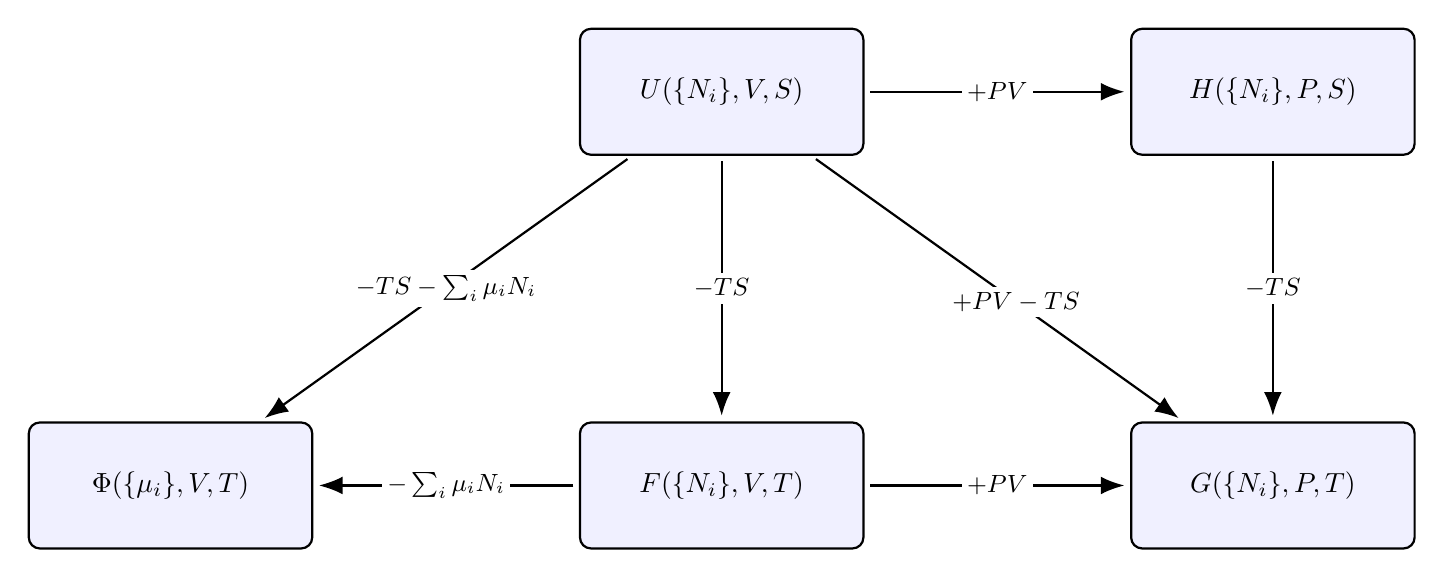
\begin{tikzpicture}[
    pot/.style={
        draw, rounded corners=4pt, thick,
        minimum width=3.6cm, minimum height=1.6cm,
        inner sep=4pt, align=center, fill=blue!6
    },
    arr/.style={-{Latex[length=3mm]}, thick, shorten >=2pt, shorten <=2pt},
    lbl/.style={fill=white, inner sep=2pt, font=\small}
]

% Nodes: U and F on the central axis, H/G on the right, Phi mirrored on the left
\node[pot] (U)   at (0,5)    {$U(\{N_i\},V,S)$};
\node[pot] (F)   at (0,0)    {$F(\{N_i\},V,T)$};
\node[pot] (H)   at (7,5)    {$H(\{N_i\},P,S)$};
\node[pot] (G)   at (7,0)    {$G(\{N_i\},P,T)$};
\node[pot] (Phi) at (-7,0)   {$\Phi(\{\mu_i\},V,T)$};

% Right-hand square
\draw[arr] (U) -- node[lbl] {$+PV$} (H);
\draw[arr] (U) -- node[lbl] {$-TS$} (F);
\draw[arr] (H) -- node[lbl] {$-TS$} (G);
\draw[arr] (F) -- node[lbl] {$+PV$} (G);
\draw[arr] (U) -- node[lbl, pos=0.55] {$+PV-TS$} (G);

% Left-hand (mirrored) edges
\draw[arr] (F) -- node[lbl] {$-\sum_i \mu_i N_i$} (Phi);
\draw[arr] (U) -- node[lbl, pos=0.5] {$-TS-\sum_i \mu_i N_i$} (Phi);

\end{tikzpicture}
\end{center}

\paragraph{Summary of the ensembles.}
The table lists, for each ensemble, which variables are fixed and which are
obtained by differentiating the potential:
\begin{center}
\renewcommand{\arraystretch}{2.6}

\begin{tabular}{|c|c|c|c|c|c|}
\hline
Ensemble & $\{N_i\}VS$ & $\{N_i\}VT$ & $\{N_i\}PS$ & $\{\mu_i\}VT$ & $\{N_i\}PT$ \\ \hline
\shortstack{Conventional\\name}
  & \shortstack{micro-\\canonical}
  & canonical
  & \shortstack{isoenthalpic-\\isobaric}
  & \shortstack{grand\\canonical}
  & \shortstack{isothermal-\\isobaric} \\ \hline \hline
\shortstack{Thermodynamic\\potential}
  & $U$ & $F$ & $H$ & $\Phi$ & $G$ \\ \hline
$N_i$
  & fixed & fixed & fixed
  & $-\dfrac{\partial \Phi}{\partial \mu_i}$ & fixed \\ \hline
$V$
  & fixed & fixed
  & $\dfrac{\partial H}{\partial P}$ & fixed
  & $\dfrac{\partial G}{\partial P}$ \\ \hline
$S$
  & fixed & $-\dfrac{\partial F}{\partial T}$ & fixed
  & $-\dfrac{\partial \Phi}{\partial T}$
  & $-\dfrac{\partial G}{\partial T}$ \\ \hline
$\mu_i$
  & $\dfrac{\partial U}{\partial N_i}$
  & $\dfrac{\partial F}{\partial N_i}$
  & $\dfrac{\partial H}{\partial N_i}$
  & fixed
  & $\dfrac{\partial G}{\partial N_i}$ \\ \hline
$P$
  & $-\dfrac{\partial U}{\partial V}$
  & $-\dfrac{\partial F}{\partial V}$ & fixed
  & $-\dfrac{\partial \Phi}{\partial V}$ & fixed \\ \hline
$T$
  & $\dfrac{\partial U}{\partial S}$ & fixed
  & $\dfrac{\partial H}{\partial S}$ & fixed & fixed \\
  \hline
\end{tabular}
\end{center}

\subsection{Mixing Entropy and the Gibbs Paradox}

\paragraph{Setting and the two properties of the entropy.}
Let $X=(U,V,N_1,N_2)$ denote the extensive variables and
$S(X)=k_B\ln\Omega(X)$ the microcanonical entropy. We use
two properties, both understood in the thermodynamic limit.
\begin{itemize}
    \item \textbf{(P1) Superadditivity.} $S(X+Y)\ge S(X)+S(Y)$.
    Place two independent systems with variables $X$ and $Y$ next to each
    other. Each pair of microstates, one from each system, is a microstate of
    the combined system with variables $X+Y$, and distinct pairs give
    distinct microstates. Hence $\Omega(X+Y)\ge\Omega(X)\Omega(Y)$, and taking
    $k_B\ln$ gives (P1).
    \item \textbf{(P2) Homogeneity.} $S(\lambda X)=\lambda S(X)$ for
    $\lambda>0$. This is extensivity. For identical particles it holds only
    if $\Omega$ counts indistinguishable particles, that is, with the factor
    $1/N!$ included.
\end{itemize}

\paragraph{Concavity of the entropy along the composition line.}
For $\lambda\in[0,1]$, (P1) and (P2) give
\begin{align*}
    S\big(\lambda X+(1-\lambda)Y\big)
    \ \ge\ S(\lambda X)+S\big((1-\lambda)Y\big)
    = \lambda S(X)+(1-\lambda)S(Y),
\end{align*}
so $S$ is concave in $X$:
\begin{equation}
    \boxed{S\big(\lambda X+(1-\lambda)Y\big)\ \ge\ \lambda S(X)+(1-\lambda)S(Y).}
\end{equation}
Now fix the total energy $2U$, the volume $2V$, and the total particle number
$2N$. The only remaining variable is the composition, which we label by the
number $t$ of species-2 particles:
\begin{equation*}
    g(t)\equiv S(2U,\,2V,\,2N-t,\,t),\qquad t\in[0,2N].
\end{equation*}
The map $t\mapsto(2U,2V,2N-t,t)$ is affine, and a concave function composed
with an affine map is concave, so $g$ is concave. Three points on this line
matter:
\begin{align*}
    g(0)&=S(2U,2V,2N,0) &&\text{(all species 1)},\\
    g(2N)&=S(2U,2V,0,2N) &&\text{(all species 2)},\\
    g(N)&=S(2U,2V,N,N) &&\text{(half and half)}.
\end{align*}
Since $(N,N)=\tfrac12(2N,0)+\tfrac12(0,2N)$, the half-and-half state is the
midpoint of the two pure states.

\paragraph{Entropy of mixing for distinguishable species.}
Take the two systems before the partition is removed,
$X=(U,V,N,0)$ and $Y=(U,V,0,N)$, and define the entropy of mixing
\begin{equation}
    \boxed{\Delta S_{\mathrm{mix}}\equiv S(2U,2V,N,N)-S(U,V,N,0)-S(U,V,0,N)
    =g(N)-S(U,V,N,0)-S(U,V,0,N).}
\end{equation}
\emph{Step 1: concavity at the midpoint.} Applying the concavity inequality
along the line with $\lambda=\tfrac12$,
\begin{align*}
    g(N)\ \ge\ \tfrac12\,g(0)+\tfrac12\,g(2N).
\end{align*}
The right-hand side is the height of the chord joining the two end points,
at its midpoint, so the graph of $g$ does not lie below its chord.

\emph{Step 2: homogeneity at the end points.} By (P2) with $\lambda=2$,
\begin{align*}
    g(0)=S(2U,2V,2N,0)=2\,S(U,V,N,0),\qquad
    g(2N)=S(2U,2V,0,2N)=2\,S(U,V,0,N).
\end{align*}
Inserting these into the midpoint inequality gives
$g(N)\ge S(U,V,N,0)+S(U,V,0,N)$, that is,
\begin{equation}
    \boxed{\Delta S_{\mathrm{mix}}\ \ge 0.}
\end{equation}
The same result follows directly from (P1), since $X+Y=(2U,2V,N,N)$.

\paragraph{When equality holds.}
Equality in the midpoint inequality means that $g(N)$ lies on the chord. A
concave function that touches its chord at an interior point equals the chord
everywhere: if some $g(t_0)$ were strictly above the chord, concavity would
put $g(N)$ strictly above it too. Therefore
\begin{equation}
    \boxed{\Delta S_{\mathrm{mix}}=0
    \iff g \text{ is affine on } [0,2N],
    \qquad
    \Delta S_{\mathrm{mix}}>0
    \iff g \text{ is not affine.}}
\end{equation}
In particular, $\Delta S_{\mathrm{mix}}>0$ whenever $S$ is strictly concave
along the composition line.

\paragraph{Identical particles and the paradox.}
For identical particles, take $X=Y=(U,V,N)$. By (P2),
\begin{align*}
    S(2U,2V,2N)=2S(U,V,N)=S(X)+S(Y),
\end{align*}
so $\Delta S_{\mathrm{mix}}=0$ exactly. In terms of $g$: if the two
``species'' are physically identical, $S$ depends only on $N_1+N_2$, so $g$
is constant, hence affine, and the equality case applies. The difference
between the two cases is whether the composition is a genuine variable of
$S$. For distinguishable species, $g$ is not affine, and removing the
partition increases the entropy by the strictly positive amount
$\Delta S_{\mathrm{mix}}$. For identical particles, $g$ is constant and
$\Delta S_{\mathrm{mix}}=0$. No continuity is expected between the two: they
differ in what the counting $\Omega$ treats as distinct, which is why (P2)
holds for identical particles only with the $1/N!$ included.

\subsection{Gibbs-Duhem Relation}

\paragraph{The intensive variables are not independent.}
The \textcolor{blue}{Gibbs-Duhem relation} states that the intensive
variables $(T,P,\{\mu_i\})$ are not independent. Write the extensive
variables as $x=(S,V,\{N_i\})$ and their conjugates as
$\xi=(T,-P,\{\mu_i\})$, using $\xi$ as in the Legendre transformation.
Let $f$ be any thermodynamic potential, obtained from $U$ by exchanging the
variables in a set $A$ for their conjugates:
\begin{equation*}
    f=U-\sum_{a\in A}\xi_a x_a,
\end{equation*}
so that $f=U$ for $A=\varnothing$, $f=F$ for $A=\{S\}$, $f=G$ for
$A=\{S,V\}$, and so on. Wherever $f$ is differentiable in its natural
variables,
\begin{equation*}
    df=\sum_{a\notin A}\xi_a\,dx_a-\sum_{a\in A}x_a\,d\xi_a.
\end{equation*}
By the Euler relation, $U=\sum_a\xi_a x_a$, so $f$ is also
\begin{equation*}
    f=\sum_{a\notin A}\xi_a x_a,
    \qquad\text{hence}\qquad
    df=\sum_{a\notin A}\xi_a\,dx_a+\sum_{a\notin A}x_a\,d\xi_a.
\end{equation*}
Comparing the two expressions for $df$ gives
\begin{equation}
    \boxed{\sum_a x_a\,d\xi_a=S\,dT-V\,dP+\sum_i N_i\,d\mu_i=0.}
\end{equation}
The result does not depend on the choice of $A$, so it holds in every
ensemble. Of the $n$ intensive variables, only $n-1$ can be varied
independently. 

\paragraph{Why no ensemble fixes all the intensive variables.}
Exchanging all extensive variables for their conjugates, $A=\{S,V,\{N_i\}\}$,
gives the potential
\begin{equation*}
    f=U-TS+PV-\sum_i\mu_iN_i=0.
\end{equation*}
It vanishes identically by the Euler relation. Such a potential would depend
on no extensive variable at all, so nothing would fix the size of the system.
A system that exchanges energy, volume, and particles freely, with all of
$(T,P,\{\mu_i\})$ held fixed, therefore has no ensemble of its own, and
Gibbs-Duhem is the statement of this fact.
\part{Phase Transtion}
    \section{First-Order Phase Transitions and Phase Diagram}
For a given system, a \textcolor{blue}{phase} is a region of the space of natural
variables in which the thermodynamic potential is analytic: infinitely
differentiable, with no kinks or divergences. A \textcolor{blue}{phase transition}
is a point where it fails to be analytic. Strictly, such singularities appear only
in the thermodynamic limit $N\to\infty$, since the partition function of a finite
system is analytic.

We usually study phases at fixed particle numbers, pressure and temperature, for
two reasons. Experimentally, these are easy to control. Structurally, the phases
inside such a system exchange energy, volume and particles with each other, so at
equilibrium $(\{\mu_i\},P,T)$ must be equal in all phases. The natural choice of
potential is then the Gibbs free energy $G(T,P,\{N_i\})$. Because $G$ is extensive,
\begin{align*}
    G(T,P,\{N_i\}) = N\,g(T,P,\{x_i\}), \qquad x_i = N_i/N,
\end{align*}
so the total size $N$ does not affect the analyticity of $G$; only $g$ does.
What matters is the composition $\{x_i\}$, of which $C-1$ are independent for $C$ component. A phase is therefore a region of the intensive variables $(T,P,\{x_i\})$,
which span a $(C-1)+2=C+1$ dimensional space. Collecting every phase in this
space gives the \textcolor{blue}{phase diagram}.

At equilibrium, $g$ is continuous, so a phase transition is never a jump in the
potential itself. Adding $g$ as one more axis to the $(C+1)$-dimensional space
$(T,P,\{x_i\})$ gives a hypersurface $g(T,P,\{x_i\})$. A
\textcolor{blue}{first-order transition} is a crease (kink) of this hypersurface:
$g$ is continuous across it, but its first derivatives jump,
\begin{align*}
    s = -\frac{\partial g}{\partial T}, \qquad v = \frac{\partial g}{\partial P},
\end{align*}
the entropy and volume per particle. Equivalently, $S=-\partial G/\partial T$ and
$V=\partial G/\partial P$ are discontinuous, which gives a latent heat
$L = T\Delta S$ and a volume change $\Delta V$. Melting and boiling are
examples. On the transition locus the coexisting phases share the same
$(\{\mu_i\},P,T)$ but have different $s$, $v$ and composition, which is why the
transition appears as a boundary of a coexistence region in the phase diagram.

Transitions of higher order also exist: the order is the order of the lowest
derivative of $g$ that is discontinuous or singular, and for these the
hypersurface has no kink and the singularity appears in the curvature. They
include the continuous transitions, such as the ferromagnetic Curie point, where
response functions like the heat capacity diverge. We defer them to a later
section.

\subsection{Gibbs Phase Rule}

    Suppose $\mathcal{P}$ phases of a system with $C$ components coexist. At
    equilibrium all phases share the same intensive variables
    $(T,P,\mu_1,\dots,\mu_C)$, which gives $C+2$ variables. Each phase has its
    own Gibbs--Duhem relation,
    \begin{align*}
        S_\alpha\,dT - V_\alpha\,dP + \sum_i N_{i,\alpha}\,d\mu_i = 0,
        \qquad \alpha = 1,\dots,\mathcal{P},
    \end{align*}
    which gives $\mathcal{P}$ independent constraints on them. The number of
    degrees of freedom $F$ is the number of variables minus the number of
    constraints,
    \begin{align}
        \boxed{F+\mathcal{P}=C+2.}
    \end{align}
    This is the \textcolor{blue}{Gibbs phase rule}. It counts only intensive
    degrees of freedom: the amount of each phase remains free and is not counted. However, this is only applicable if $(T,P,\mu_1,\dots,\mu_C)$ are the only intensive variables. We will encounter system that depends on the magnetic field $\vec B$ of itself, which add another intensive variable to the count.

\subsection{Clapeyron Equation and Fixed-Composition ($P$--$T$) Phase Diagram}
No matter how many components the system has, temperature and pressure always
participate. Consider the $P$--$T$ plane at fixed composition $\{x_i\}$ within the
$(C+1)$-dimensional phase diagram. In this slice only $(P,T)$ can vary, so there
are $2$ degrees of freedom. Two phases $1$ and $2$ coexist when every chemical
potential matches,
\begin{equation*}
    \mu_i^{(1)}(T,P) = \mu_i^{(2)}(T,P), \qquad i=1,\dots,C,
\end{equation*}
which relates $P$ and $T$ and reduces the degrees of freedom from $2$ to $1$.
The coexistence locus is therefore a curve in the plane. Moving along it, the two
phases keep equal chemical potentials, so $d\mu_i^{(1)}=d\mu_i^{(2)}$ and, by
the Gibbs--Duhem relation at fixed composition,
\begin{equation*}
    -s_1\,dT + v_1\,dP = -s_2\,dT + v_2\,dP ,
\end{equation*}
which gives the \textcolor{blue}{Clapeyron equation}
\begin{equation}
    \boxed{\frac{dP}{dT}=\frac{\Delta s}{\Delta v}}, \qquad
    \Delta s = s_2-s_1,\;\; \Delta v = v_2-v_1 .
\end{equation}
At coexistence the transition proceeds reversibly at fixed $T$ and $P$, so the
latent heat per particle is $\ell = T\Delta s$, and
\begin{equation}
    \boxed{\frac{dP}{dT}=\frac{\ell}{T\,\Delta v}.}
\end{equation}

Now suppose a third phase $3$ also coexists. Then
\begin{equation*}
    \mu_i^{(1)}(T,P)=\mu_i^{(2)}(T,P)=\mu_i^{(3)}(T,P), \qquad i=1,\dots,C .
\end{equation*}
Each pair of phases has its own coexistence curve, $\mu^{(1)}=\mu^{(2)}$,
$\mu^{(2)}=\mu^{(3)}$ and $\mu^{(1)}=\mu^{(3)}$. A point lying on the first two
satisfies $\mu^{(1)}=\mu^{(2)}=\mu^{(3)}$, so it lies on the third as well:
only two of the three conditions are independent. Two independent equations in the
two unknowns $(T,P)$ leave no degrees of freedom, so three phases can coexist
only at an isolated point, the \textcolor{blue}{triple point}, where the three
two-phase curves, the \textcolor{blue}{triple curves} intersect.

\subsection{Unary System}
A \textcolor{blue}{unary system} has only one component, $C=1$. This is a special case of the
fixed-composition slice, since the composition is always $x=1$. We discuss it
because it is the building block of higher-dimensional phase diagrams and
introduces some terminology. For $C=1$ the phase rule reads
$F = 3-\mathcal{P}$, so the number of coexisting phases $\mathcal{P}$ fixes the
number of free variables.

Within a single phase ($\mathcal{P}=1$, $F=2$), $P$ and $T$ can both be varied
freely. The system is said to be in \textcolor{blue}{bivariant equilibrium}.

When two phases coexist ($\mathcal{P}=2$, $F=1$), only one of $P$ and $T$ can be
varied freely; the other is then fixed by the Clapeyron relation $P=P(T)$. The
system is said to be in \textcolor{blue}{univariant equilibrium}, and the locus
of two-phase coexistence is called a \textcolor{blue}{univariant curve}.

When three phases coexist ($\mathcal{P}=3$, $F=0$), no variable can be changed
freely. The system is said to be in \textcolor{blue}{invariant equilibrium}, and
the point where this happens is called an \textcolor{blue}{invariant point}
(the triple point).

    
    \section{Binary System}

\subsection{The $X$--$P$--$T$ Diagram}
A \textcolor{blue}{binary system} has two components, $C=2$, so its composition is described by one
independent variable, $X=x_2$ with $x_1=1-X$. The phase diagram is therefore
three-dimensional in $(P,T,X)$. One can picture it as stacking the fixed-composition
$P$--$T$ diagrams and varying $X$ bit by bit. The phase rule reads
$F=4-\mathcal{P}$, and each unary structure is stretched by one dimension.

\begin{itemize}
    \item \textcolor{blue}{Tervariant volume} ($\mathcal{P}=1$, $F=3$). The bivariant regions of the
    unary diagram become volumes, where $P$, $T$ and $X$ can all be varied freely
    without changing phase. The cross section of such a volume changes with $X$.
    \item \textcolor{blue}{Bivariant surface} ($\mathcal{P}=2$, $F=2$). The univariant curves become
    surfaces. Two coexisting phases generally have different compositions, so each
    phase has its own bivariant surface, and the two surfaces are joined by tie
    lines. The region they enclose is the two-phase region, where the overall
    composition fixes the amount of each phase.
    \item \textcolor{blue}{Univariant curve} ($\mathcal{P}=3$, $F=1$). The invariant points become
    curves, along which only one variable can be varied freely. Three bivariant
    surfaces, one for each pair of phases, meet along each such curve.
    \item \textcolor{blue}{Invariant point} ($\mathcal{P}=4$, $F=0$). A new kind of invariant point
    appears, where none of $P$, $T$ or $X$ can be varied. Every subset of the four
    phases can coexist near it, so it is where $\binom{4}{3}=4$ univariant curves,
    $\binom{4}{2}=6$ two-phase (bivariant) surfaces and $\binom{4}{1}=4$
    single-phase (tervariant) volumes meet. Therefore, it is also called the \textcolor{blue}{quadruple point.}
\end{itemize}

\part{Classical thermodnynamic}

\part{Physical Chemistry}

\part{Quantum Statistical Mechanics}

\end{document}